En un reactor de mezcla perfecta lo  que  se  consigue  es  que  exista  una  homogeneidad 
perfecta en la reacción, es decir, que todos los puntos tengan la misma temperatura y presión, 
consiguiendo que toda la mezcla que se extraiga tenga idénticas condiciones a la que 
está en el interior del reactor.
	
	En el menú principal, encontramos dos botones dentro del apartado de reactores de mezcla perfecta. Estos dos botones serán utilizados indistintamente en función del propósito que tengamos: cálculo del volumen o cálculo de la conversión.
	
\section{Cálculo del volumen}
Si seleccionamos la opción de cálculo de volumen, nos aparece una ventana como la que se puede observar en la Figura \ref{fig:ventana_volumen}.

\begin{figure}[h!]
	\begin{center}
		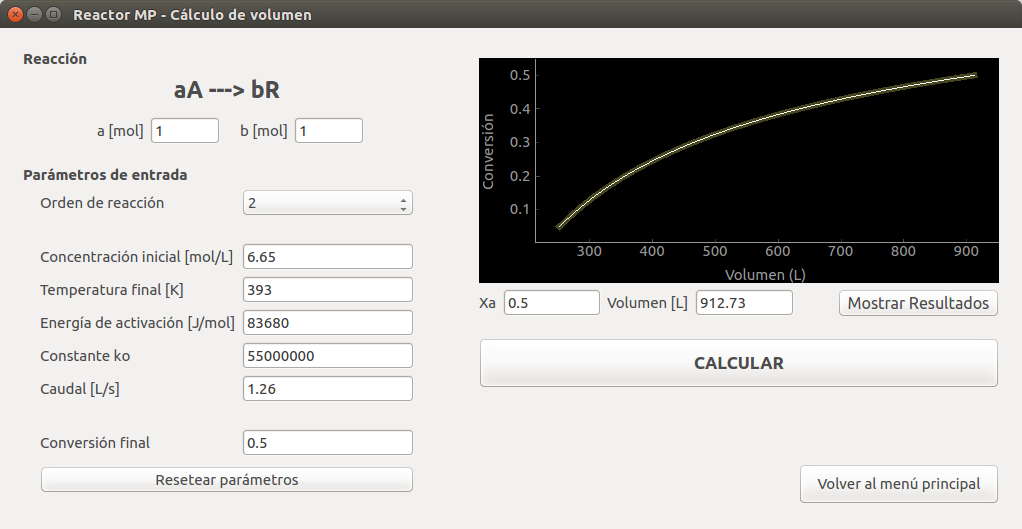
\includegraphics[width=0.85\textwidth]{./imagenes/reactor_fp/mezcla_perfecta1.png}\caption{Ventana reactor MP (cálculo de volumen)}\label{fig:ventana_volumen}
	\end{center}
\end{figure}

En la parte superior izquierda, el programa nos indica el tipo de reacción con la que vamos a trabajar y permite modificar el número de reactivos y productos. Una vez que hayamos establecido la reacción deseada, deberemos seleccionar el orden de reacción en el desplegable e introducir todos los parámetros de entrada indicados, prestando especial atención a las unidades en las que se indican que han de ser introducidos.

Cuando tengamos introducidos todos los datos indicados, podremos obtener el resultado final pulsando sobre el botón \textbf{'CALCULAR'}, situado en la parte derecha de la ventana. Inmediatamente después de pulsar sobre dicho botón el programa representará de forma gráfica el resultado en la parte derecha de la ventana, y se indicará el valor final obtenido como resultado, en función de nuestros parámetros de entrada, en las celdas situadas en la parte inferior del gráfico.

Si deseamos visualizar el gráfico en una ventana independiente ((Figura \ref{fig:ventana_graficas_volumen})), podemos hacerlo pulsado sobre el botón \textbf{'Mostrar Resultados'}. En esta nueva ventana, no solo podremos ver el mismo gráfico descrito anteriormente, sino que además dispondremos de un cursor que nos permitirá ver el resultado en cada punto de la curva. En esta nueva ventana también se nos permite exportar el gráfico como una imagen.

\begin{figure}[h!]
	\begin{center}
		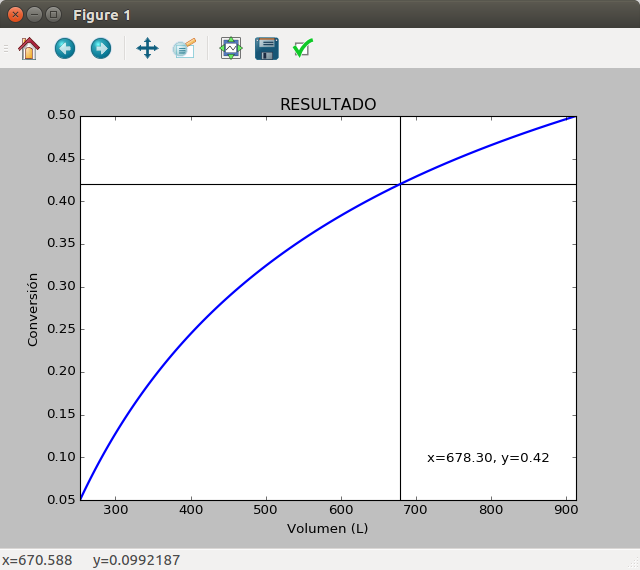
\includegraphics[width=0.85\textwidth]{./imagenes/reactor_fp/mezcla_perfecta2.png}\caption{Ventana de resultados reactor MP (cálculo de volumen)}\label{fig:ventana_graficas_volumen}
	\end{center}
\end{figure}

Finalmente, podemos realizar un borrado de todas las celdas, mediante el botón \textbf{'Resetear parámetros'}, para realizar un nuevo cálculo. Si no deseamos realizar más cálculos y queremos regresar al menú principal, podremos hacerlo pinchando sobre el botón \textbf{'Volver al menú principal'} de abajo a la derecha de la ventana.


\section{Cálculo de la conversión}
Si seleccionamos la opción de cálculo de la conversión, nos aparece una ventana como la que se puede observar en la Figura \ref{fig:ventana_conversion}.

\begin{figure}[h!]
	\begin{center}
		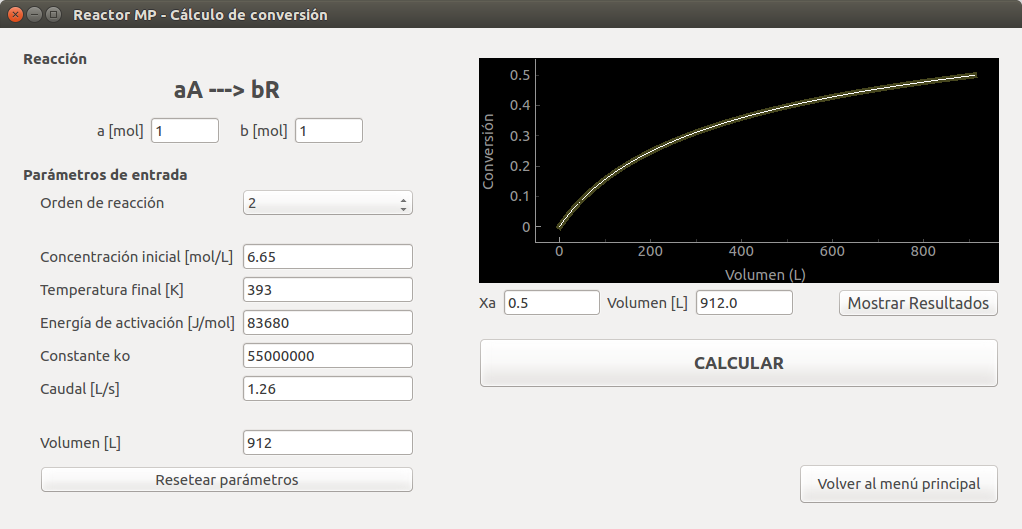
\includegraphics[width=0.85\textwidth]{./imagenes/reactor_fp/mezcla_perfecta3.png}\caption{Ventana reactor MP (cálculo de conversión)}\label{fig:ventana_conversion}
	\end{center}
\end{figure}

Al igual que para el cálculo del volumen descrito anteriormente, se nos informa en la parte superior izquierda de la ventana sobre el tipo de reacción con la que vamos a trabajar y se nos permite modificar el número de reactivos y productos. Una vez realizadas estas operaciones, seleccionaremos el orden de reacción en el desplegable y a continuación introduciremos todos los parámetros de entrada indicados, prestando especial atención a las unidades en las que se indican que han de ser introducidos.

Podremos obtener el resultado final, una vez que hayamos introducido todos los datos, pulsando sobre el botón \textbf{'CALCULAR'} situado en la parte derecha de la ventana. Así se representará el resultado en el gráfico de la parte derecha de la ventana. Además, los resultados numéricos obtenidos como solución final, en función de nuestros parámetros de entrada, se mostrarán en las celdas situadas en la parte inferior del gráfico mencionado.

Si deseamos ver los resultados en una ventana independiente (Figura \ref{fig:ventana_graficas_conversion}) bastará con pulsar sobre el botón \textbf{'Mostrar Resultados'}. En esta nueva ventana, como en el caso anterior, dispondremos de un cursor que nos permitirá movernos a través de la curva obtenida para ver el resultado en cada punto concreto. En esta nueva ventana también se nos permite exportar el gráfico como una imagen.

\begin{figure}[h!]
	\begin{center}
		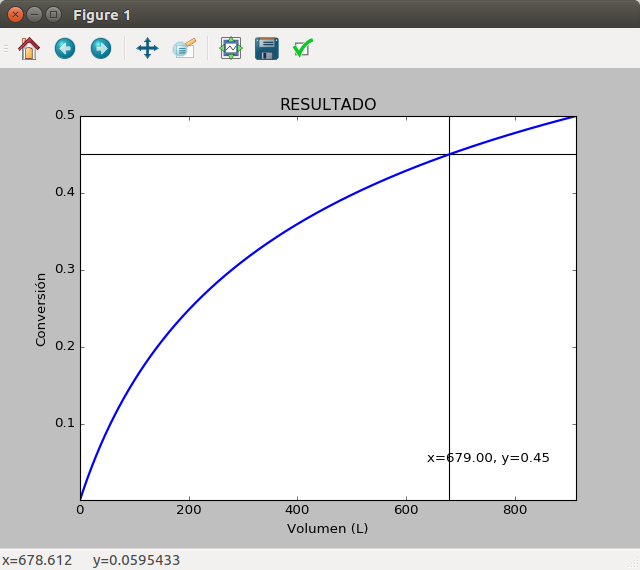
\includegraphics[width=0.85\textwidth]{./imagenes/reactor_fp/mezcla_perfecta4.png}\caption{Ventana de resultados reactor MP (cálculo de conversión)}\label{fig:ventana_graficas_conversion}
	\end{center}
\end{figure}

Finalmente, podemos realizar un borrado de todas las celdas, mediante el botón \textbf{'Resetear parámetros'}, para realizar un nuevo cálculo. Si no deseamos realizar más cálculos y queremos regresar al menú principal, podremos hacerlo mediante el botón \textbf{'Volver al menú principal'}, situado en la parte inferior derecha de la ventana.